\documentclass{article}
\usepackage[top=3cm, bottom=3cm, left = 2cm, right = 2cm]{geometry} 
\geometry{a4paper} 
\usepackage[T1]{polski}
\usepackage[utf8]{inputenc}
\usepackage{titling}
\usepackage{caption}
\usepackage{algorithm}
\usepackage{algpseudocode}
\usepackage[parfill]{parskip}
\usepackage{multirow}
\usepackage{graphicx}
\usepackage{pgfplots}
\usepackage{stmaryrd}
\usepackage{textcomp}
\usepackage{amsmath}
\usepackage{amsfonts}

\renewcommand\maketitlehooka{\null\mbox{}\vfill}
\renewcommand\maketitlehookd{\vfill\null}

\floatname{algorithm}{Algorytm}
\algrenewcommand\algorithmicrequire{\textbf{Input:}}
\algrenewcommand\algorithmicensure{\textbf{Output:}}

\title{Metody Optymalizacji}
\author{Karol Janic}
\date{1 maja 2025}

\begin{document}

\begin{titlingpage}
    \maketitle
\end{titlingpage}

\tableofcontents

\newpage

\section{Zadanie 1}
\subsection{Cel}
Celem zadania jest zaplanowanie produkcji desek w tartatu w taki sposób aby zminimalzować liczbę odpadów.
Deski mają stałą szerokośc i należy poprzecinać je w taki sposób aby zaspokoić zapotrzebowanie klientów na deski, które mogą być krótsze.

\subsection{Model}
Model parametryzowany jest szerokością desek $L \in \mathbb{R}_+$ (w calach), z której produkowane są wyroby oraz zapotrzebowaniem wyrażonym ciągiem par $(l_i, n_i)$, gdzie $1 \leq i \leq N$, $l_i$ jest szerokością deski a $n_i$ ich liczbą.
Cięcia te generowane są przy użyciu rekurencyjnego algorytmu, który w każdym kroku sprawdza czy szerokość deski jest większa od $l_i$ i jeżeli tak to odejmuje $l_i$ od szerokości deski i wywołuje się rekurencyjnie na pozostałej szerokości deski.

\subsubsection{Generowanie możliwych cięć}
W fazie preprocesingu generowane są wszystkie możliwe cięcia, które mogą być wykonane na desce o szerokości $L$.
Numerujemy je od $1$ do $M$. Przez $C_m^r$ oznaczamy liczbę odpadów a $C_m^{l_i}$ liczbę desek $l_i$ w cięciu $m$-tym.

\subsubsection{Zmienne decyzyjne}
Całkowitoliczbowe zmienne decyzyjne $x_m$, gdzie $1 \leq m \leq M$ o wartościach nieujemnych określają dla każdego możliwego cięcia liczbę desek pociętych w ten sposób.

\subsubsection{Funkcja celu}
Funkcją celu jest minimalizacja sumy odpadów po cięciach i sumy długości desek wyprodukowanych ponad zapotrzebowanie:
\begin{align*}
    \sum_{m=1}^{M} x_m \cdot C_m^r + \sum_{i=1}^{N} \left(\sum_{m=1}^{M} x_m \cdot C_m^{l_i} - n_i\right) \cdot l_i
\end{align*}

\subsubsection{Ograniczenia}
Jedyna grupa ograniczeń wymusza spełnienie zapotrzebowania na każdą szerokośc deski:
\begin{align*}
    \sum_{m=1}^M C_m^{l_i} \leq n_i, \qquad \qquad \qquad 1 \leq i \leq N
\end{align*}

\subsection{Dane}
Zadana została długość deski $L = 22$ oraz zapotrzebowanie w tabeli \ref{tab:zad1a}.
\begin{table}[h]
    \centering
    \begin{minipage}{0.45\textwidth}
        \centering
        \begin{tabular}{l|ccc}
            $i$ & 1 & 2 & 3 \\
            \hline
            $l_i$ & 3 & 5 & 7 \\
            \hline
            $n_i$ & 80 & 120 & 110 \\
        \end{tabular}
        \caption{Zapotrzebowanie na deski}
        \label{tab:zad1a}
    \end{minipage}
    \hfill
    \begin{minipage}{0.45\textwidth}
        \centering
        \begin{tabular}{ccc|c}
            \multicolumn{3}{c|}{Cięcie} & Liczba sztuk \\
            3 & 5 & 7 & \\
            \hline
            5 & 0 & 1 & 9 \\
            1 & 1 & 2 & 37 \\
            0 & 3 & 1 & 28 \\
        \end{tabular}
        \caption{Wyznaczone cięcia i liczby sztuk}
        \label{tab:zad1b}
    \end{minipage}
\end{table}

\subsection{Wyniki}
Zapisano model programowania liniowego i wyznaczono optymalne rozwiązanie dla danych. 
Wyniki przedstawiono w tabeli \ref{tab:zad1b}. Taka produkcja generuje 18 cali odpadów. 
Łatwo sprawdzić, że jest to rozwiązanie dopuszczalne, ponieważ każde zapotrzebowanie zostało spełnione.

\section{Zadanie 2}
\subsection{Cel}
Celem zadania jest zaplanowanie kolejności wykonywania zadań na jednej maszynie w taki sposób aby zminimalizować sumę czasu zakończenia wszystkich zadań przemnożoną przez ich wagi.
Dodatkowo każde zadanie ma czas najwcześniejszego rozpoczęcia, który musi być spełniony.

\subsection{Model}
Model parametryzowany jest liczbą zadań $N \in \mathbb{N}_+$ czasami ich wykonania $p_i \in \mathbb{R}$, wagami $w_i \in \mathbb{R}$ oraz czasami najwcześniejszego ich rozpoczęcia $r_i \in \mathbb{R}$, gdzie $1 \leq i \leq N$.

\subsubsection{Zmienne decyzyjne}
Nieujemne zmienne decyzyjne $x_i$, gdzie $1 \leq i \leq N$ określają czas rozpoczęcia $i$-tego zadania.
Dodatkowo binarne zmienne decyzyjne $y_{ij}$, gdzie $1 \leq i,j \leq N$ określają kolejność wykonywania zadań - 1 jeżeli zadanie $i$ jest przed zadaniem $j$ oraz 0 w przeciwnym przypadku.

\subsubsection{Funkcja celu}
Funkcją celu jest minimalizacja sumy czasów zakończenia wszystkich zadań przemnożoną przez ich wagi:
\begin{align*}
    \sum_{i=1}^{N} w_i \cdot (x_i + p_i)
\end{align*}

\subsubsection{Ograniczenia}
Pierwsza grupa ograniczeń wymusza spełnienie czasów najwcześniejszego rozpoczęcia zadań:
\begin{align*}
    x_i \geq r_i, \qquad \qquad \qquad 1 \leq i \leq N
\end{align*}

Druga grupa ograniczeń wymusza, że kolejność wykonywania zadań jest spójna:
\begin{align*}
    y_{ii} = 0, \qquad &&1 \leq i \leq N \\
    y_{ij} + y_{ji} = 1, \qquad &&1 \leq i<j \leq N
\end{align*}

Ostatnia grupa ograniczeń wymusza, że każde zadanie może być rozpoczęte tylko po zakończeniu poprzedniego:
\begin{align*}
    x_i + p_i \leq x_j + M \cdot (1 - y_{ij}), \qquad &&1 \leq i<j \leq N \\
    x_j + p_j \leq x_i + M \cdot y_{ij}, \qquad &&1 \leq i<j \leq N
\end{align*}
gdzie $M$ jest dużą liczbą - w tym przypadku $ \displaystyle M = \max_{1 \leq i \leq N}{r_i} + \sum_{i=1}^{N} p_i + 1$.
Jest ono wykorzystywane do zamodelowania implikacji, że jeżeli zadanie $i$ jest przed zadaniem $j$ to zadanie $j$ może być rozpoczęte tylko po zakończeniu zadania $i$.

\newpage

\subsection{Dane}
Zadane zostały czasy wykonania $p_i$, wagi $w_i$ oraz czasy gotowości $r_i$ dla 10 zadań, które przedstawione są w tabeli \ref{tab:zad2}.
\begin{table}[h]
    \centering
    \begin{minipage}{0.45\textwidth}
        \centering
        \begin{tabular}{c|c|c|c}
            Zadanie $i$ & Czas ($p_i$) & Waga ($w_i$) & Gotowość ($r_i$) \\
            \hline
            1 & 4 & 5 & 0 \\
            2 & 3 & 2 & 2 \\
            3 & 2 & 7 & 5 \\
            4 & 6 & 4 & 3 \\
            5 & 5 & 1 & 7 \\
            6 & 1 & 9 & 0 \\
            7 & 7 & 3 & 4 \\
            8 & 2 & 6 & 6 \\
            9 & 3 & 8 & 1 \\
            10 & 4 & 2 & 8 \\
        \end{tabular}
        \caption{Parametry zadań: $p_i$, $w_i$, $r_i$}
        \label{tab:zad2}
    \end{minipage}
    \hfill
    \begin{minipage}{0.45\textwidth}
        \centering
        \begin{tabular}{c|c|c}
            Zadanie & Rozpoczęcie & Zakończenie \\
            \hline
            6 & 0 & 1 \\
            9 & 1 & 4 \\
            3 & 5 & 7 \\
            8 & 7 & 9 \\
            1 & 9 & 13 \\
            2 & 13 & 16 \\
            4 & 16 & 22 \\
            10 & 22 & 26 \\
            7 & 26 & 33 \\
            5 & 33 & 38 \\
        \end{tabular}
        \caption{Czasy rozpoczęcia i zakończenia zadań}
        \label{tab:zad2b}
    \end{minipage}
\end{table}

\subsection{Wyniki}
Zapisano model programowania liniowego i wyznaczono optymalne rozwiązanie dla danych.
Optymalna kolejność wykonywania zadań została przedstawiona w tabeli \ref{tab:zad2b}.
Koszt całkowity wynosi 518 jednostki. Łatwo sprawdzić, że jest to rozwiązanie dopuszczalne, ponieważ każde zadanie zostało rozpoczęte po jego czasie gotowości i trwało odpowiednio długo.

\section{Zadanie 3}
\subsection{Cel}
Celem zadania jest zaplanowanie kolejności wykonywania zadań na wielu maszynach w taki sposób aby zminimalizować czas zakończenia wszystkich zadań. Dodatkowo każde zadanie ma określoną listę poprzedników, które muszą być zakończone przed jego rozpoczęciem.

\subsection{Model}
Model parametryzowany jest liczbą maszyn $M \in \mathbb{N}_+$, liczbą zadań $N \in \mathbb{N}_+$, czasami ich wykonania $p_i \in \mathbb{R}$ oraz listą poprzedników zadań $P_i \subseteq \{1,2,\ldots,N\}$, gdzie $1 \leq i \leq N$.

\subsubsection{Zmienne decyzyjne}
Nieujemne zmienne decyzyjne $x_i$, gdzie $1 \leq i \leq N$ określają czas rozpoczęcia $i$-tego zadania. 
Binarne zmienne decyzyjne $y_{m,i,j}$, gdzie $1 \leq m \leq M$, $1 \leq i,j \leq N$ określają kolejność wykonywania zadań - 1 jeżeli zadanie $i$ jest przed zadaniem $j$ oraz 0 w przeciwnym przypadku.
Binarne zmienne decyzyjne $a_{m,i}$, gdzie $1 \leq m \leq M$ oraz $1 \leq i \leq N$ określają czay na $m$-tej maszynie wykonywane jest $i$-te zadanie.
Dodatkowo jest zmienna decyzyjna $t \in \mathbb{R}$, która określa czas zakończenia wszystkich zadań.

\subsubsection{Funkcja celu}
Funkcją celu jest minimalizacja czasu zakończenia wszystkich zadań $t$.

\subsubsection{Ograniczenia}
Pierwsza grupa ograniczeń wymusza przypisanie zadania do tylko jednej maszyny:
\begin{align*}
    \sum_{m=1}^{M} a_{m,i} = 1, \qquad \qquad \qquad 1 \leq i \leq N
\end{align*}

Druga grupa ograniczeń wymusza, że każde zadanie może być rozpoczęte tylko po zakończeniu poprzedników:
\begin{align*}
    x_i \geq x_p + p_p, \qquad &&1 \leq i \leq N, p \in P_i \\
\end{align*}

Każde zadanie musi być zakończone przed czasem $t$:
\begin{align*}
    x_i + p_i \leq t, \qquad \qquad \qquad 1 \leq i \leq N
\end{align*}

Ostatnia grupa ograniczeń zapewnia, że zadania na jednej maszynie nie mogą się nakładać:
\begin{align*}
    x_i + p_i \leq x_j + M \cdot (1 - y_{m,i,j}) + M \cdot (2 - a_{m,i} - a_{m,j}), \qquad &&1 \leq i<j \leq N, 1 \leq m \leq M \\
    x_j + p_j \leq x_i + M \cdot y_{m,i,j} + M \cdot (2 - a_{m,i} - a_{m,j}), \qquad &&1 \leq i<j \leq N, 1 \leq m \leq M
\end{align*}
gdzie $M$ jest dużą liczbą - w tym przypadku $ \displaystyle M = \sum_{i=1}^{N} p_i + 1$.
Jest ono wykorzystywane do zamodelowania implikacji, że jeżeli zadanie $i$ jest przed zadaniem $j$ to zadanie $j$ może być rozpoczęte tylko po zakończeniu zadania $i$ oraz czy zadania $i$ i $j$ są przypisane do tej samej maszyny $m$.

\subsection{Dane}
Zadane zostały $M = 3$ maszyny oraz $N = 9$ zadań, które mają czasy wykonania i listy poprzedników jak w tabeli \ref{tab:zad3a}.
\begin{table}[h]
    \centering
    \begin{minipage}{0.4\textwidth}
        \centering
        \begin{tabular}{c|c|l}
            Zadanie & Czas trwania & Poprzednicy \\
            \hline
            1 & 1 & --- \\
            2 & 2 & --- \\
            3 & 1 & --- \\
            4 & 2 & 1, 2, 3 \\
            5 & 1 & 2, 3 \\
            6 & 1 & 4 \\
            7 & 3 & 4, 5 \\
            8 & 6 & 5 \\
            9 & 2 & 6, 7 \\
        \end{tabular}
        \caption{Zadania z czasem trwania i poprzednikami}
        \label{tab:zad3a}
    \end{minipage}
    \hfill
    \begin{minipage}{0.4\textwidth}
        \centering
        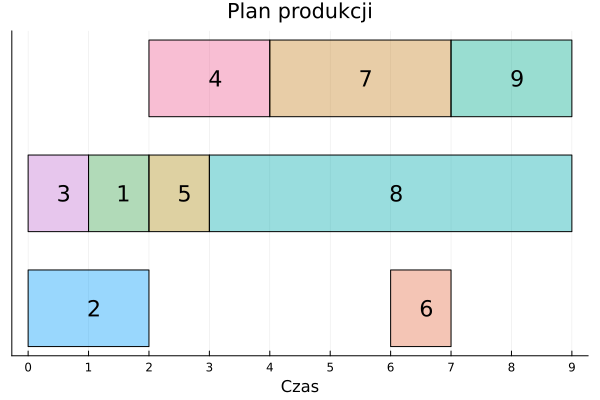
\includegraphics[width=\linewidth]{../produkcja_na_wielu_maszynach/wynik.png}
        \captionof{figure}{Wizualizacja zależności między zadaniami na wielu maszynach}
        \label{fig:zad3b}
    \end{minipage}
\end{table}

\subsection{Wyniki}
Zapisano model programowania liniowego i wyznaczono optymalne rozwiązanie dla danych.
Optymalna kolejność wykonywania zadań została przedstawiona na rysunku \ref{fig:zad3b}.
Czas zakończenia wszystkich zadań wynosi 9 jednostek czasu.
Porównując wyznaczone zależności z tabelką \ref{tab:zad3a} można sprawdzić że rozwiązanie jest dopuszczalne, ponieważ każde zadanie zostało rozpoczęte po zakończeniu poprzedników i trwało odpowiednio długo.

\section{Zadanie 4}
\subsection{Cel}
Celem zadania jest rozdzielenie zasobów do zadań w taki sposób aby zminimalizować całkowity czas zakończenia wszystkich zadań.
Każde zadanie ma określone wymagania na zasoby, czas ich wykonania oraz listę poprzedników, które muszą być zakończone przed jego rozpoczęciem.

\subsection{Model}
Model parametryzowany jest specifikacją zasobów i zadań. Każde z $R$ zasobów ma określony swój limit $r_i$, gdzie $1 \leq i \leq R$.
Każde z $N$ zadań ma zadany swój czas wykonania $p_i \in \mathbb{R}$, wymagania na zasoby $w_{r} \in \mathbb{N}_+$ oraz listę poprzedników $P_i \subseteq \{1,2,\ldots,N\}$, gdzie $1 \leq i \leq N$ oraz $1 \leq r \leq R$.

\subsubsection{Zmienne decyzyjne}
Nieujemne zmienne decyzyjne $t_i$, gdzie $1 \leq i \leq N$ określają momenty rozpoczęcia pewnego zadania - jednego lub wielu.
Binarne zmienne decyzyjne $x_{i,e}$, gdzie $1 \leq i,e \leq N$ określają czy zadanie $i$ jest aktywne w momencie $e$-tym. Zmienna $t_{\mathrm{MAX}} \in \mathbb{R}_+$ określa czas zakończenia wszystkich zadań. 

\subsubsection{Funkcja celu}
Funkcją celu jest minimalizacja czasu zakończenia wszystkich zadań $t_{\mathrm{MAX}}$.

\subsubsection{Ograniczenia}
Pierwsza grupa ograniczeń wymusza przypisanie każdego zadania do conajmniej jednego momentu, aby każde zadanie zostało wykonane:
\begin{align*}
    \sum_{e=1}^{N} x_{i,e} \geq 1, \qquad \qquad \qquad 1 \leq i \leq N
\end{align*}

Druga grupa ograniczeń wymusza monotoniczność czasów momentów:
\begin{align*}
    t_{i} = 0, \qquad \qquad \qquad \qquad i=1 \\
    t_{i} \geq t_{i-1}, \qquad \qquad \qquad 2 \leq i < N
\end{align*}

Trzecia grupa ograniczeń wyznacza czas zakończenia każdego zadania:
\begin{align*}
    t_{\mathrm{MAX}} >= t_{e} + (x_{i,e} - x_{i,e-1}) \cdot p_i, \qquad &&1 \leq i,e \leq N
\end{align*}

Kolejna grupa ograniczeń zapewnia czas trwania każdego zadania:
\begin{align*}
    t_{j} \geq t_{i} + p_i \cdot (x_{i,e} - x_{i,e-1} - x_{j,e} + x_{j,e-1}), \qquad &&1 \leq i,j \leq N, 1 \leq e \leq N
\end{align*}

Następna grupa zadań zapewnia ciągłość zadań w czasie:
\begin{align*}
    \sum_{f=1}^{e-1} x_{i,f} \geq M \cdot (1 - x_{i,e} + x_{i,e-1}), \qquad &&1 \leq i \leq N, 2 \leq e \leq N \\
    \sum_{f=e}^{N} x_{i,f} \geq M \cdot (1 + x_{i,e} - x_{i,e-1}), \qquad &&1 \leq i \leq N, 2 \leq e \leq N
\end{align*}

Przedostatnia grupa ograniczeń wymusza, że każde zadanie może być rozpoczęte tylko po zakończeniu poprzedników:
\begin{align*}
    x_{p,e} + \sum_{f=1}^{e} x_{i,f} \geq 1 + M \cdot (1 - x_{i,e}), \qquad &&1 \leq i \leq N, p \in P_i, 1 \leq e \leq N
\end{align*}

Ostatnia grupa ograniczeń wymusza, że w żadnym momencie nie można przekroczyć limitu zasobów:
\begin{align*}
    \sum_{i=1}^{N} w_{r} \cdot x_{i,e} \leq r_r, \qquad &&1 \leq r \leq R, 1 \leq e \leq N
\end{align*}
\subsection{Dane}
Zadane zostały $R = 1$ zasób z limitem $r_1 = 30$ oraz $N = 8$ zadań, które mają czasy wykonania, wymagania na zasoby i listy poprzedników jak w tabeli \ref{tab:zad4a}.
\begin{table}[h]
    \centering
    \begin{minipage}[t]{0.4\textwidth}
        \centering
        % Tabela zadań
        \begin{tabular}{c|c|l|c}
            Zadanie & Czas & Poprzednicy & Zapotrzebowanie \\
            \hline
            1 & 50 & ---     & 1: 9 \\
            2 & 47 & 1       & 1: 17 \\
            3 & 55 & 1       & 1: 11 \\
            4 & 46 & 1       & 1: 4 \\
            5 & 32 & 2       & 1: 13 \\
            6 & 57 & 3, 4    & 1: 7 \\
            7 & 15 & 4       & 1: 7 \\
            8 & 62 & 5, 6, 7 & 1: 17 \\
        \end{tabular}
        \caption{Zadania z czasem, poprzednikami i zapotrzebowaniem}
        \label{tab:zad4a}
    \end{minipage}
    \hfill
    \begin{minipage}{0.4\textwidth}
        \centering
        % \vspace{0.5cm}
        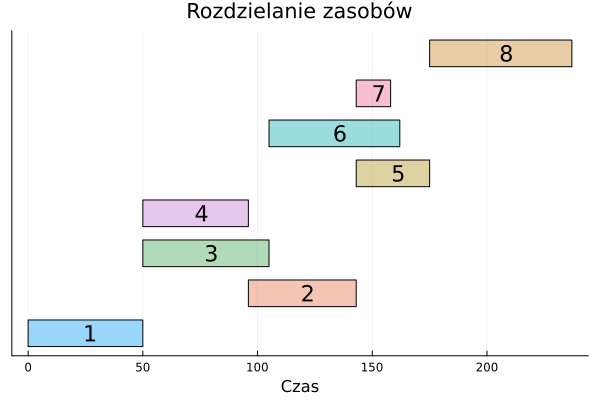
\includegraphics[width=\linewidth]{../rozdzielanie_zasobow/wynik.png}
        \captionof{figure}{Wizualizacja rozdziału zasobów do zadań}
        \label{fig:zad4b}
    \end{minipage}
\end{table}

\subsection{Wyniki}
Zapisano model programowania liniowego i wyznaczono optymalne rozwiązanie dla danych.
Optymalna kolejność wykonywania zadań została przedstawiona na rysunku \ref{fig:zad4b}.
Porównując wyznaczone zależności z tabelką \ref{tab:zad4a} można sprawdzić że rozwiązanie jest dopuszczalne, ponieważ każde zadanie zostało rozpoczęte po zakończeniu poprzedników i trwało odpowiednio długo. 
Dodatkowo w żadnym momencie nie przekroczono limitu zasobów. Całkowity czas zakończenia wszystkich zadań wynosi 237 jednostek czasu.

\end{document}
